\documentclass[10pt,a4paper,margin=0pt]{scrartcl}
\usepackage[naustrian]{babel}
\usepackage[utf8]{inputenc}
\usepackage{fancyhdr}
\usepackage{graphicx}
\usepackage{pdfpages}
\usepackage{listings}
\usepackage{enumitem}
\usepackage{booktabs}
\usepackage{graphicx}
\usepackage{a4wide}
\usepackage{listingsutf8}
\usepackage{float}
\usepackage{hyperref}

%Listing-Formatierung
\definecolor{mygreen}{RGB}{0,100,0}
\lstset{
  basicstyle=\ttfamily,
  showspaces=false, showstringspaces=false,
  tabsize=2, breaklines,
  keywordstyle=\color{blue}\bfseries,
  commentstyle=\color{mygreen},
  stringstyle=\color{red},
  title=\lstname
}
\lstdefinestyle{sharpc}{language=[Sharp]C, frame=single, rulecolor=\color{blue!80!black}}
\fancyhf{}
\lhead{Simon Guschlbauer}
\chead{\textbf{WEA5}}
\rhead{\today}
\cfoot{\thepage}
\pagestyle{fancy}

\begin{document}
\fontsize{10pt}{24pt}\selectfont
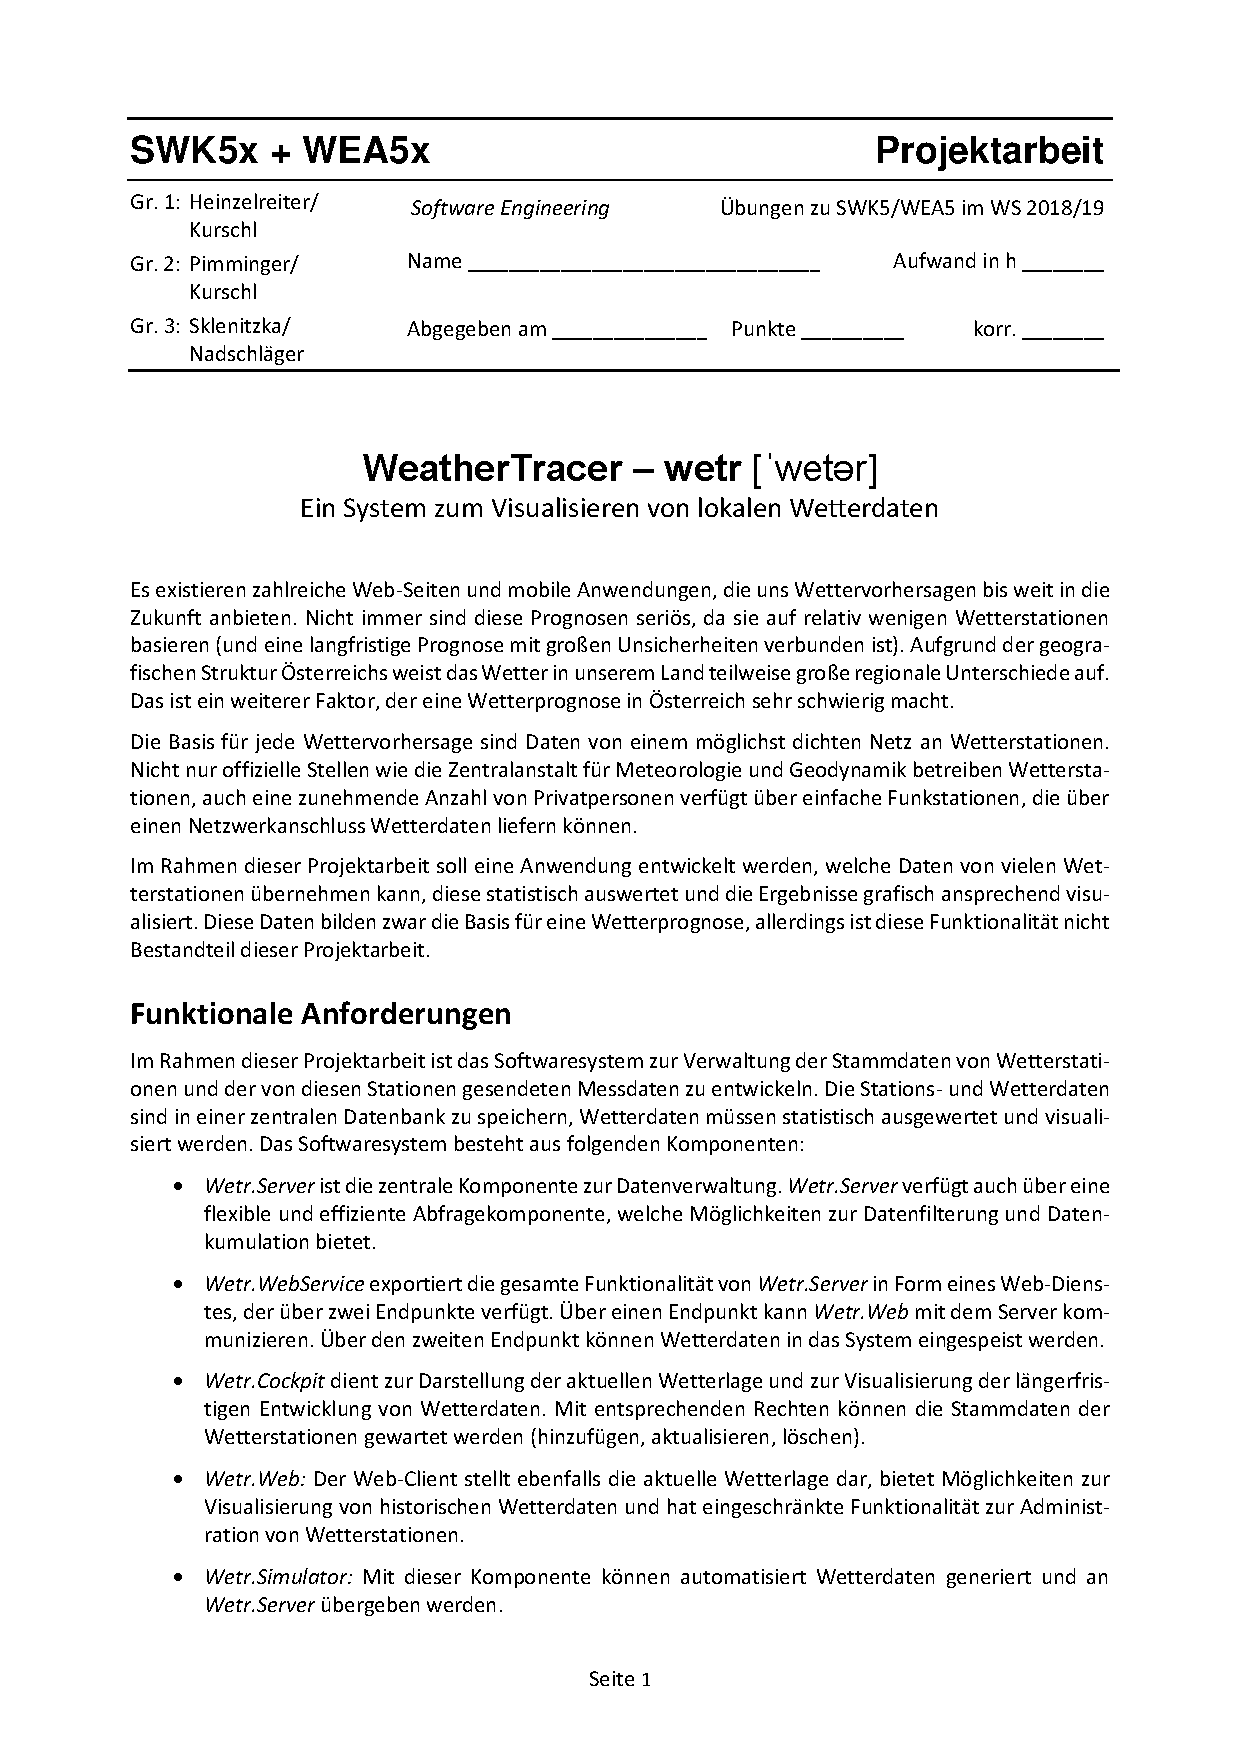
\includepdf[pages=-]{Projekt-SWK5-WEA5-VZ}
\section{Installation}
\subsection{Voraussetzungen}
\begin{itemize}
	\item NPM
	\item Angular CLI
\end{itemize}
\subsection{Verwendete Technologien}
\begin{itemize}
	\item \href{https://getbootstrap.com/}{Bootstrap}
	\item \href{https://mdbootstrap.com/docs/angular/>}{Material Design for Bootstrap}
	\item \href{https://fontawesome.com//}{Font Awesome}
\end{itemize}
\subsection{Inbetriebnahme}
Um das Projekt in Betrieb zu nehmen muss zunächst \textit{npm install} durchgeführt werden um die benötigten Packete zu installieren. Danach kann mit \textit{ng serve} die Angular Anwendung gestartet werden. Standardmäßig ist die Andwendung dann unter \url{http://localhost:4200/} erreichbar.\\\\
Die Adresse des zu verwendenden REST-Services kann in der Datei api-configuration.ts festgelegt werden. Standardmäßig ist dort \url{http://localhost:54405} hinterlegt.\\\\
\textbf{Achtung}\\
Um den Service ordnungsgemäß zu verwenden muss eine entsprechender REST-Service eingetragen und verfügbar sein.
\pagebreak
\section{Architektur}
\pagebreak
\section{Services}
Die Services uns Modelklassen wurden automatisch aus dem vom REST-Service zur Verfügung gestellten swagger.json generiert. Deswegen ist die Namensgebung und Codestruktur nicht optimal.
\subsection{measuremen-service}
\begin{itemize}
	\item MeasurementGetMeasurementForStation(...)\\
	Führt eine einfache Abfrage der Messungen für eine Station durch
	\item MeasurementGetAccumulationForStation(...)\\
	Führt eine akkumulierte Abfrage der Messungen für eine Station durch
	\item MeasurementInsert(...)\\
	Gibt eine neu erstelle Messungen an den REST-Service weiter.
\end{itemize}
\subsection{user-service}
\begin{itemize}
	\item UserLogin(params: UserLoginParams)\\
	Nimmt Benutzername und Passwort entgegen und gibt diese an den REST-Service weiter.
\end{itemize}
\pagebreak
\subsection{station-service}
\begin{itemize}
	\item StationGetAllStations(...)\\
	Fragt alle Stationen ab.
	\item StationInsert(...)\\
	Fügt eine neue Station ein
	\item StationUpdate(...)\\
	Ändert eine bestehende Station
	\item StationDelete(...)\\
	Löscht eine bestehende Station
	\item StationGetById(...)\\
	Fragt Station nach Stations-Id ab
	\item StationGetByCommunity(...)\\
	Fragt Stationen nach Gemeinde ab
	\item StationGetByUsernameName(...)\\
	Fragt Stationen nach Ersteller ab
	\item StationGetCommunities(...)\\
	Fragt alle Gemeinden ab 
\end{itemize}

\pagebreak
\section{Komponenten}
\subsection{Home}
Diese Komponente stellt den Einstiegspunkt in die Anwendung dar. Von hier aus sind alle wichtigen Bereiche der Anwendung erreichbar. Außerdem wird nach man nach dem Ausloggen wieder auf diesen Bereich weitergeleitet.
\begin{figure}[H]
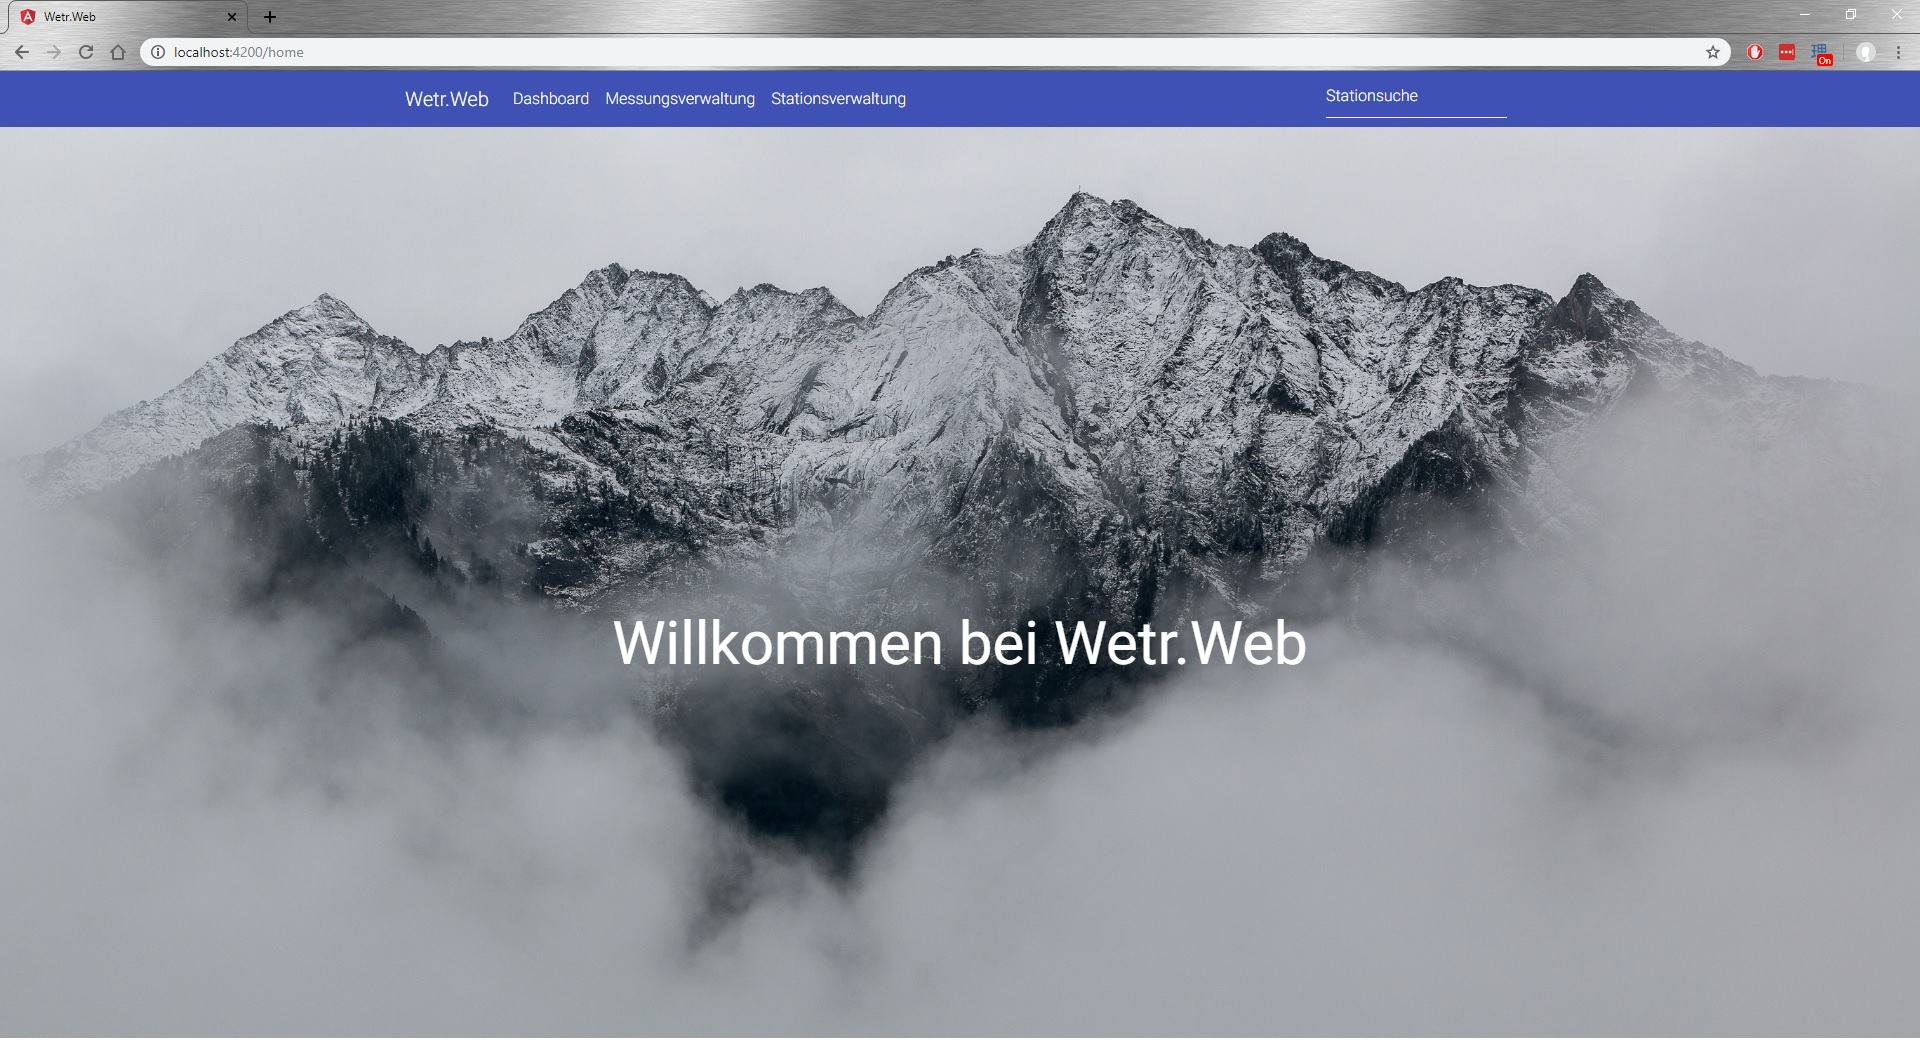
\includegraphics[width=\textwidth]{./img/home.jpg}
\centering
\end{figure}
\subsection{Header}
Die Header-Komponenten ist immer sichtbar und beinhaltet die Navigation sowie die öffentliche Stationssuche.
\pagebreak
\subsection{Search}
Die Search-Komponente ist in die Header-Komponente integriert und kann von jedem Benutzer verwendet werden um nach Stationen zu suchen und die Detailseiten der Stationen aufzurufen.
\begin{figure}[H]
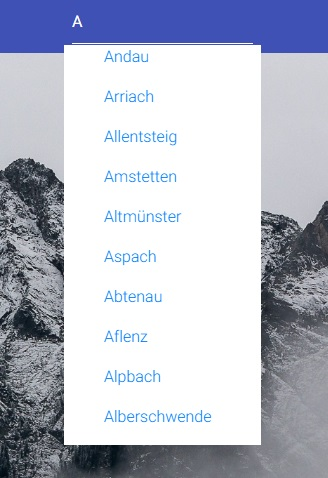
\includegraphics[scale=0.5]{./img/suche.jpg}
\centering
\end{figure}
\subsection{Dashboard}
Die Dashboard-Komponente ist nur für eingeloggte Benutzer verfügbar und zeigt die aktuelle Temperatur sowie Links zu den vorher favorisierten Stationen des Benutzers an.
\begin{figure}[H]
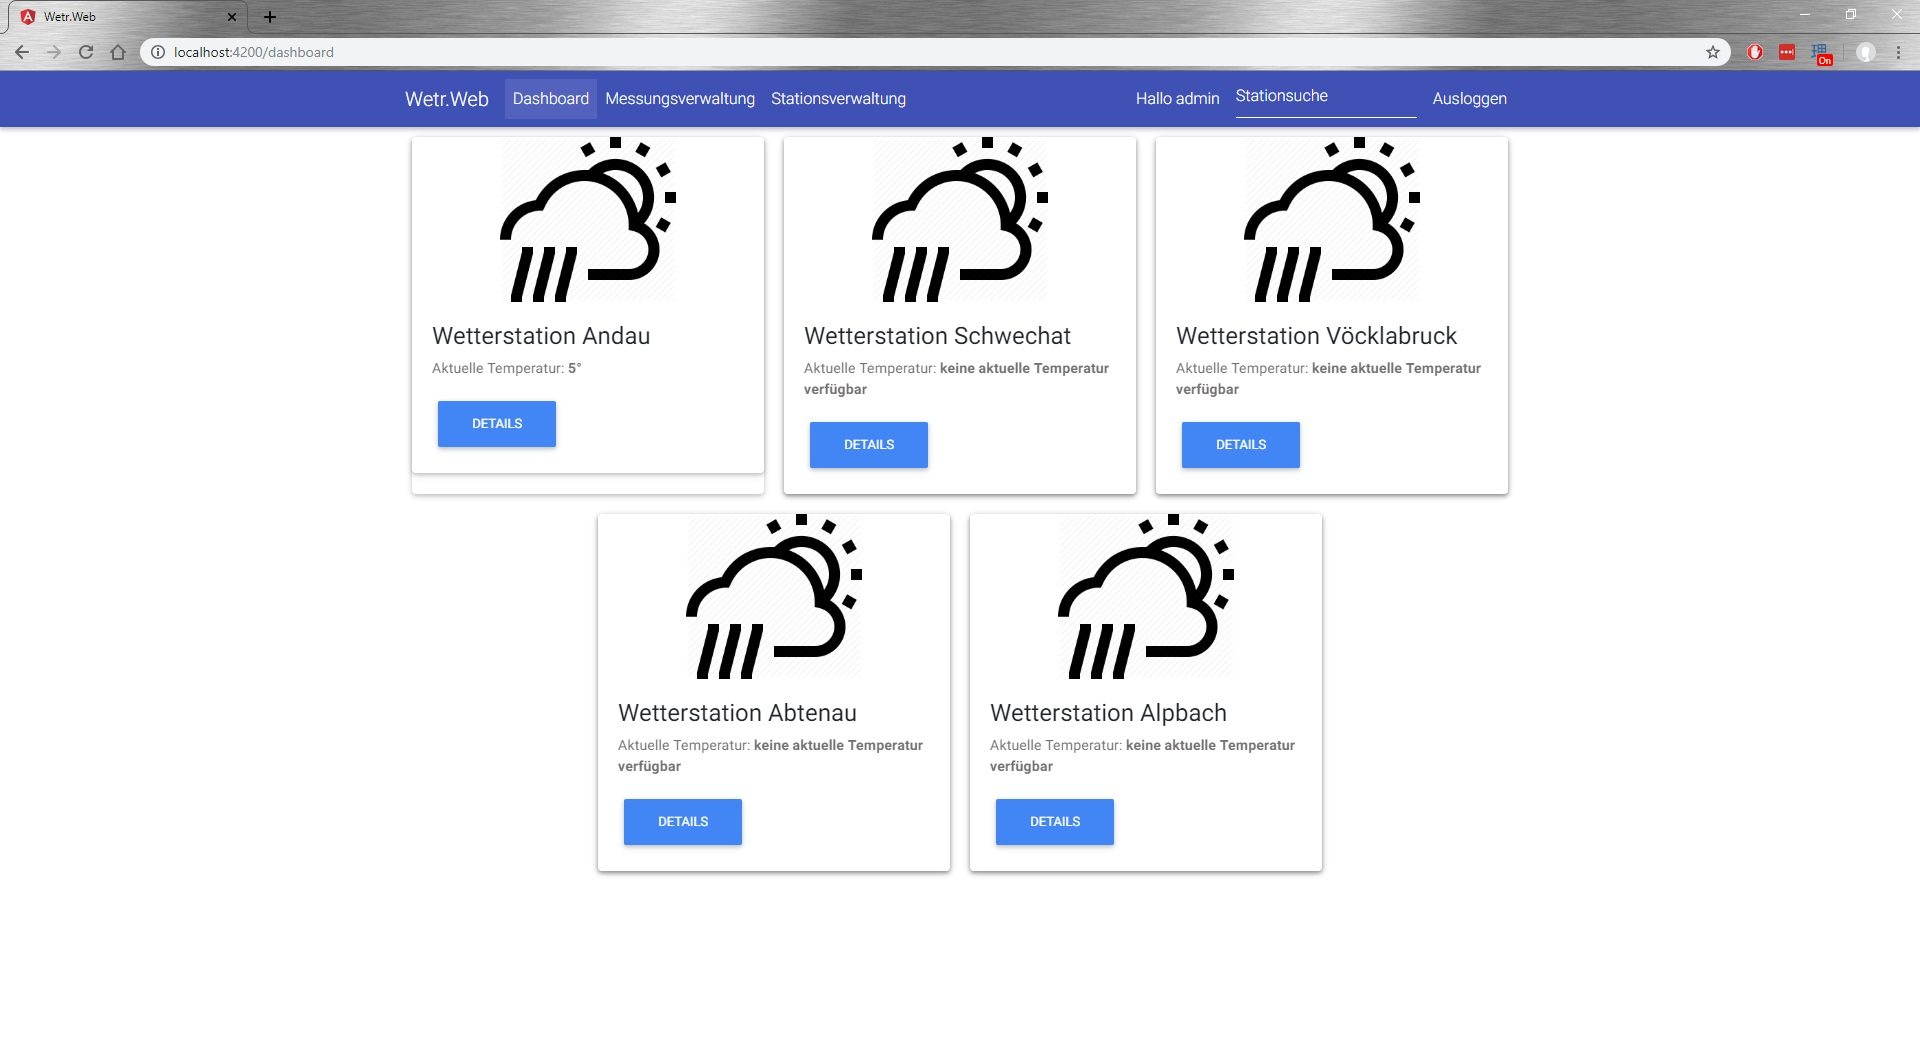
\includegraphics[width=\textwidth]{./img/dashboard.jpg}
\centering
\end{figure}
\subsection{Measurement-Management}
Diese Komponente dient dazu um neue Messungen anzulegen. Sollten die Angaben nicht korrekt sein weißen Hinweismeldung darauf hin und der Button kann nicht gedrückt werden. Nach erfolgreichem Absenden gibt eine weitere Hinweismeldung dem Benutzer Feedback über den Status der Operation.
\begin{figure}[H]
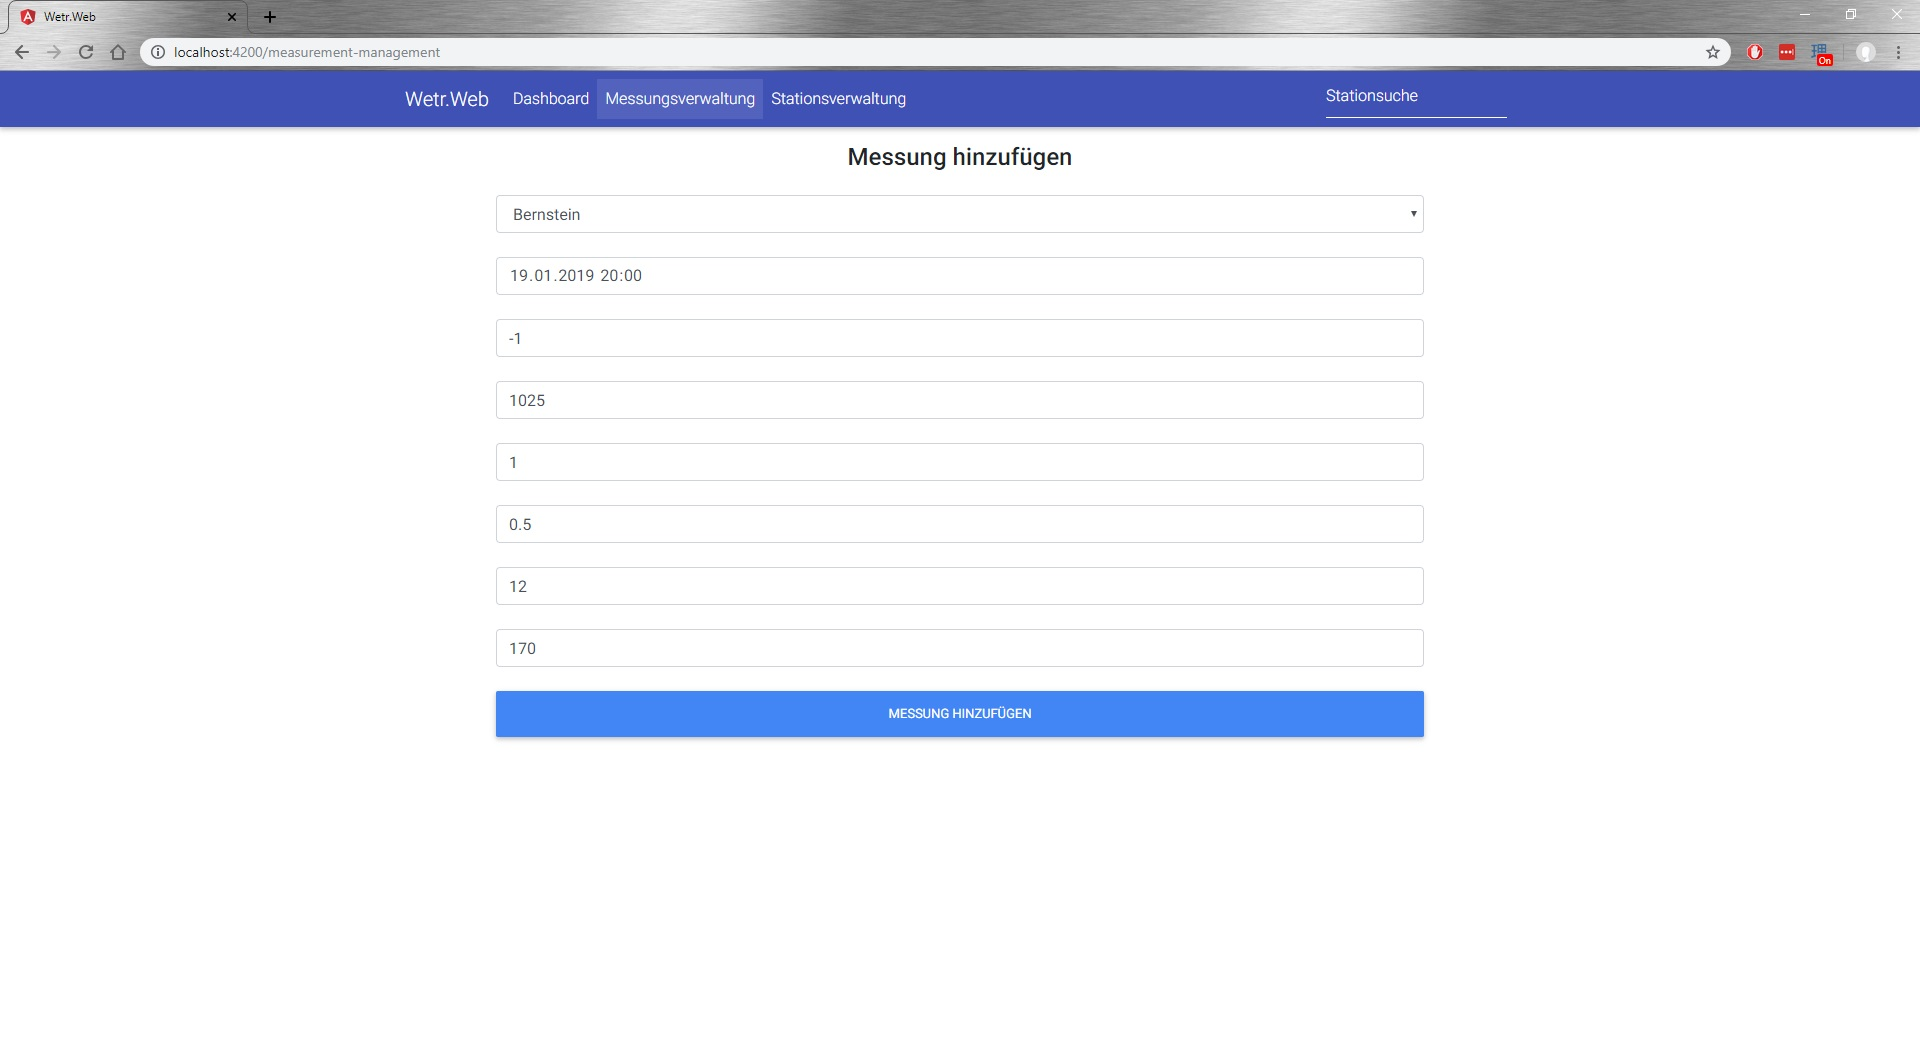
\includegraphics[width=\textwidth]{./img/messung.jpg}
\centering
\end{figure}
\begin{figure}[H]
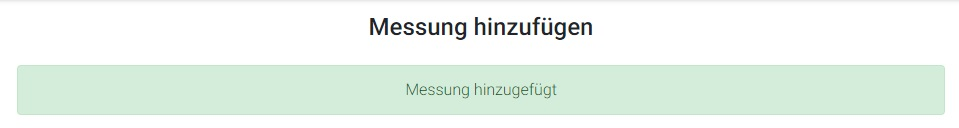
\includegraphics[width=\textwidth]{./img/messung1.jpg}
\centering
\end{figure}
\pagebreak
\subsection{Station-Management}
Diese Komponente dient dazu um bestehende Stationen zu ändern oder zu löschen. Außerdem kann man von hier aus zur Seite "Station anlegen" navigieren.
\begin{figure}[H]
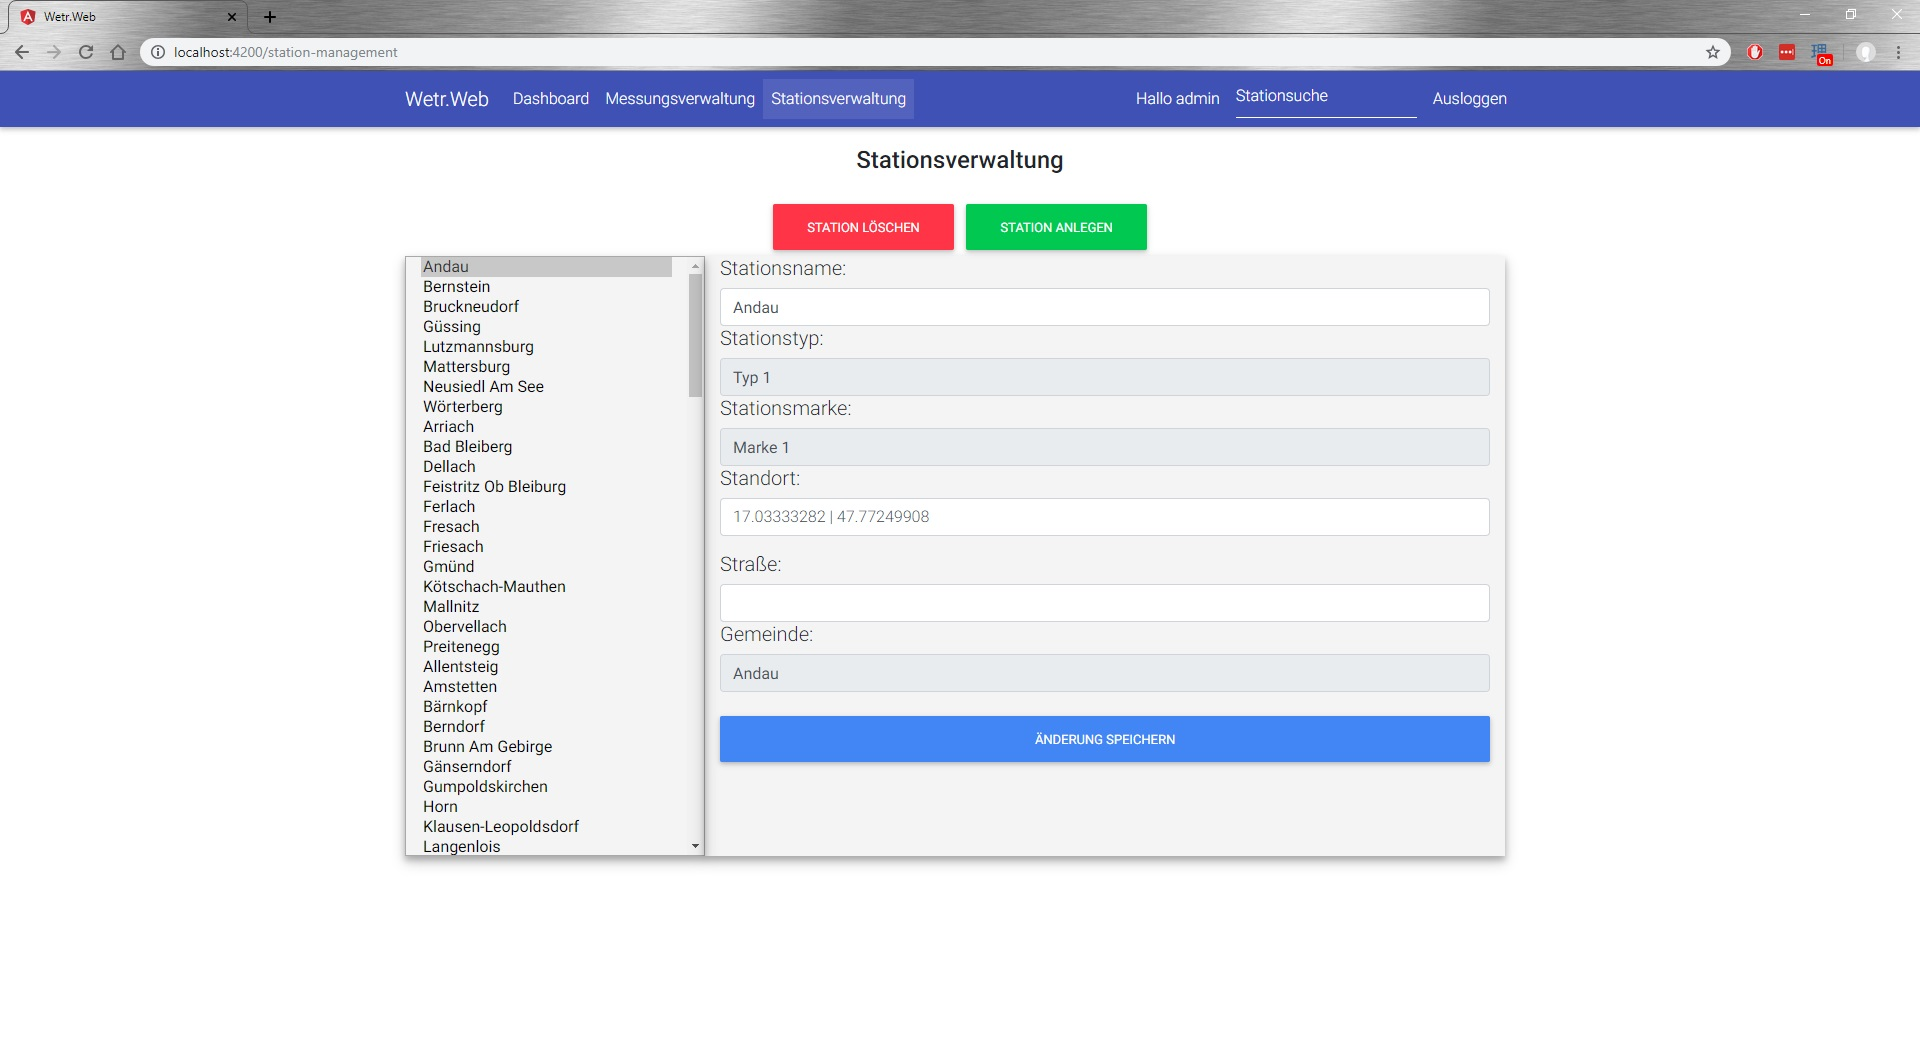
\includegraphics[width=\textwidth]{./img/station-management.jpg}
\centering
\end{figure}
\subsection{Create-Station}
Diese Komponente dient dazu um neue Stationen anzulegen.
\begin{figure}[H]
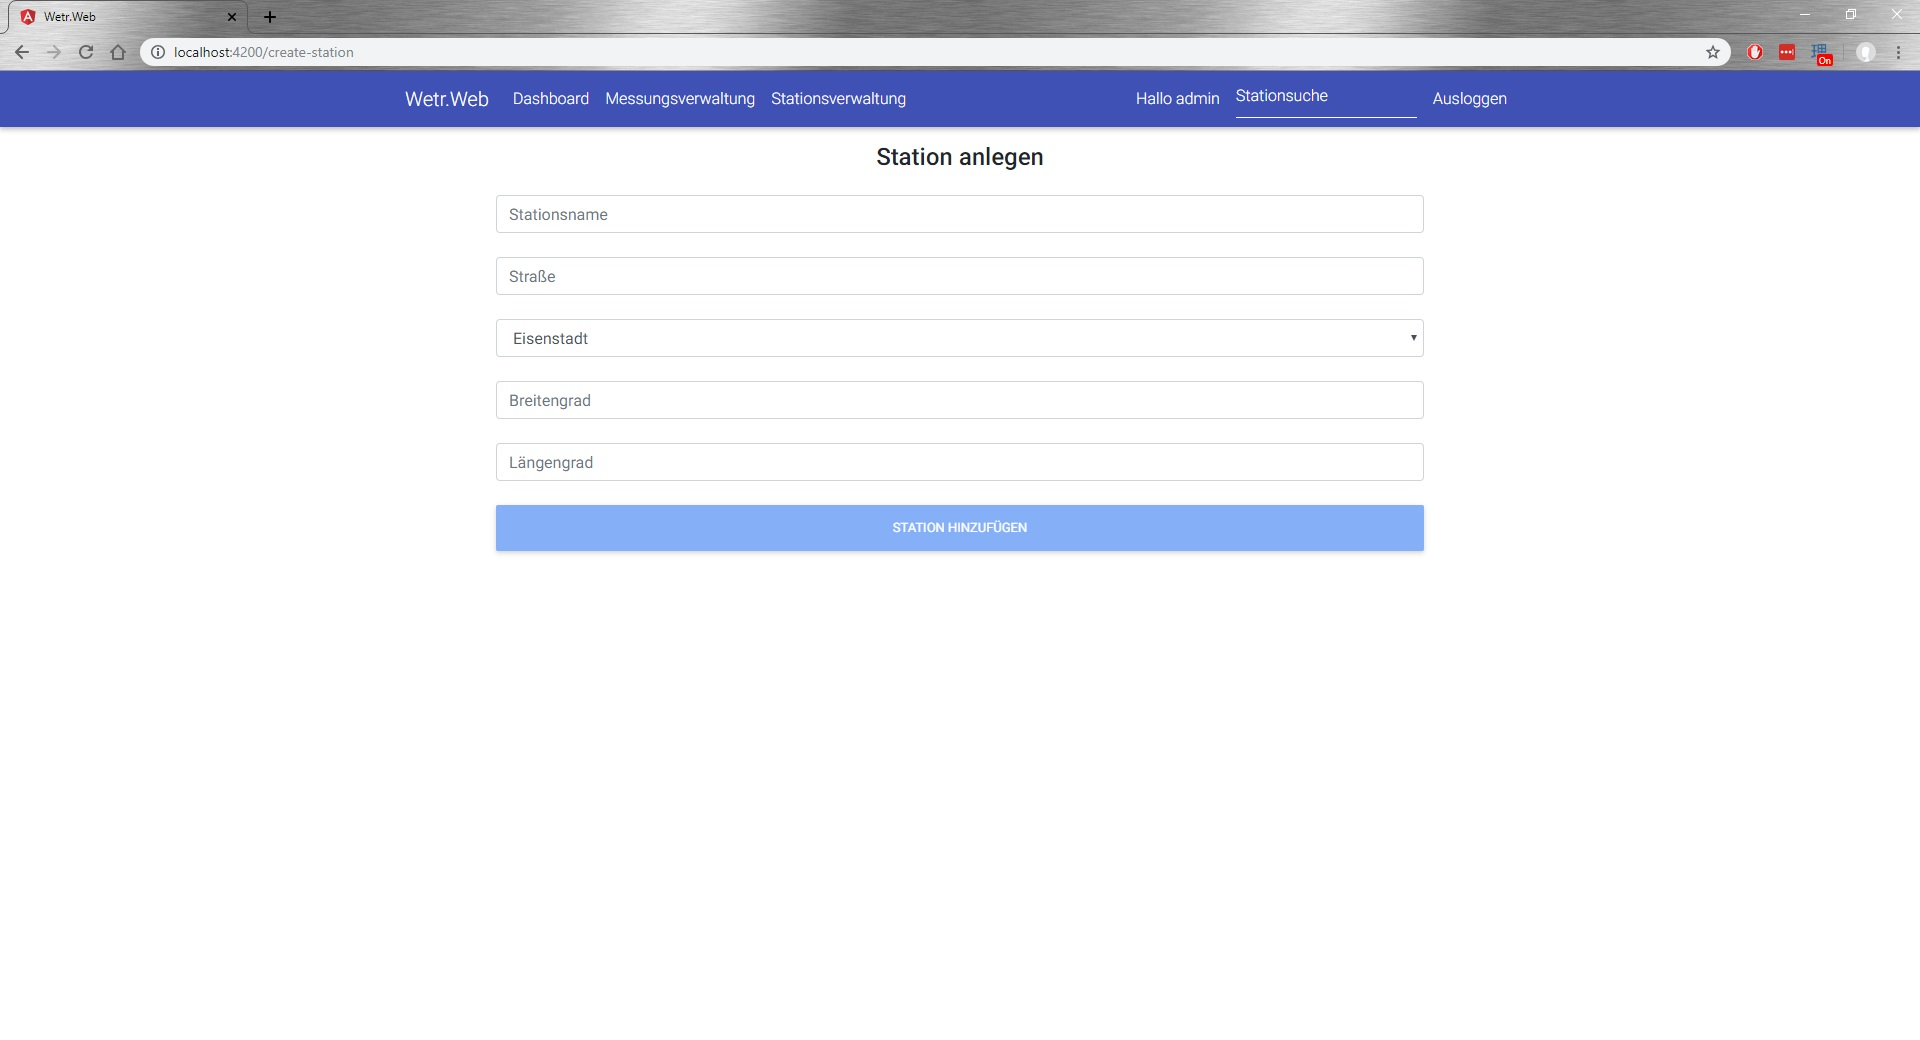
\includegraphics[width=\textwidth]{./img/station-add.jpg}
\centering
\end{figure}
\subsection{Station-Details}
Zeigt alle Daten zu einer Station an sowie Messungsdaten zu dieser Station.
\begin{figure}[H]
	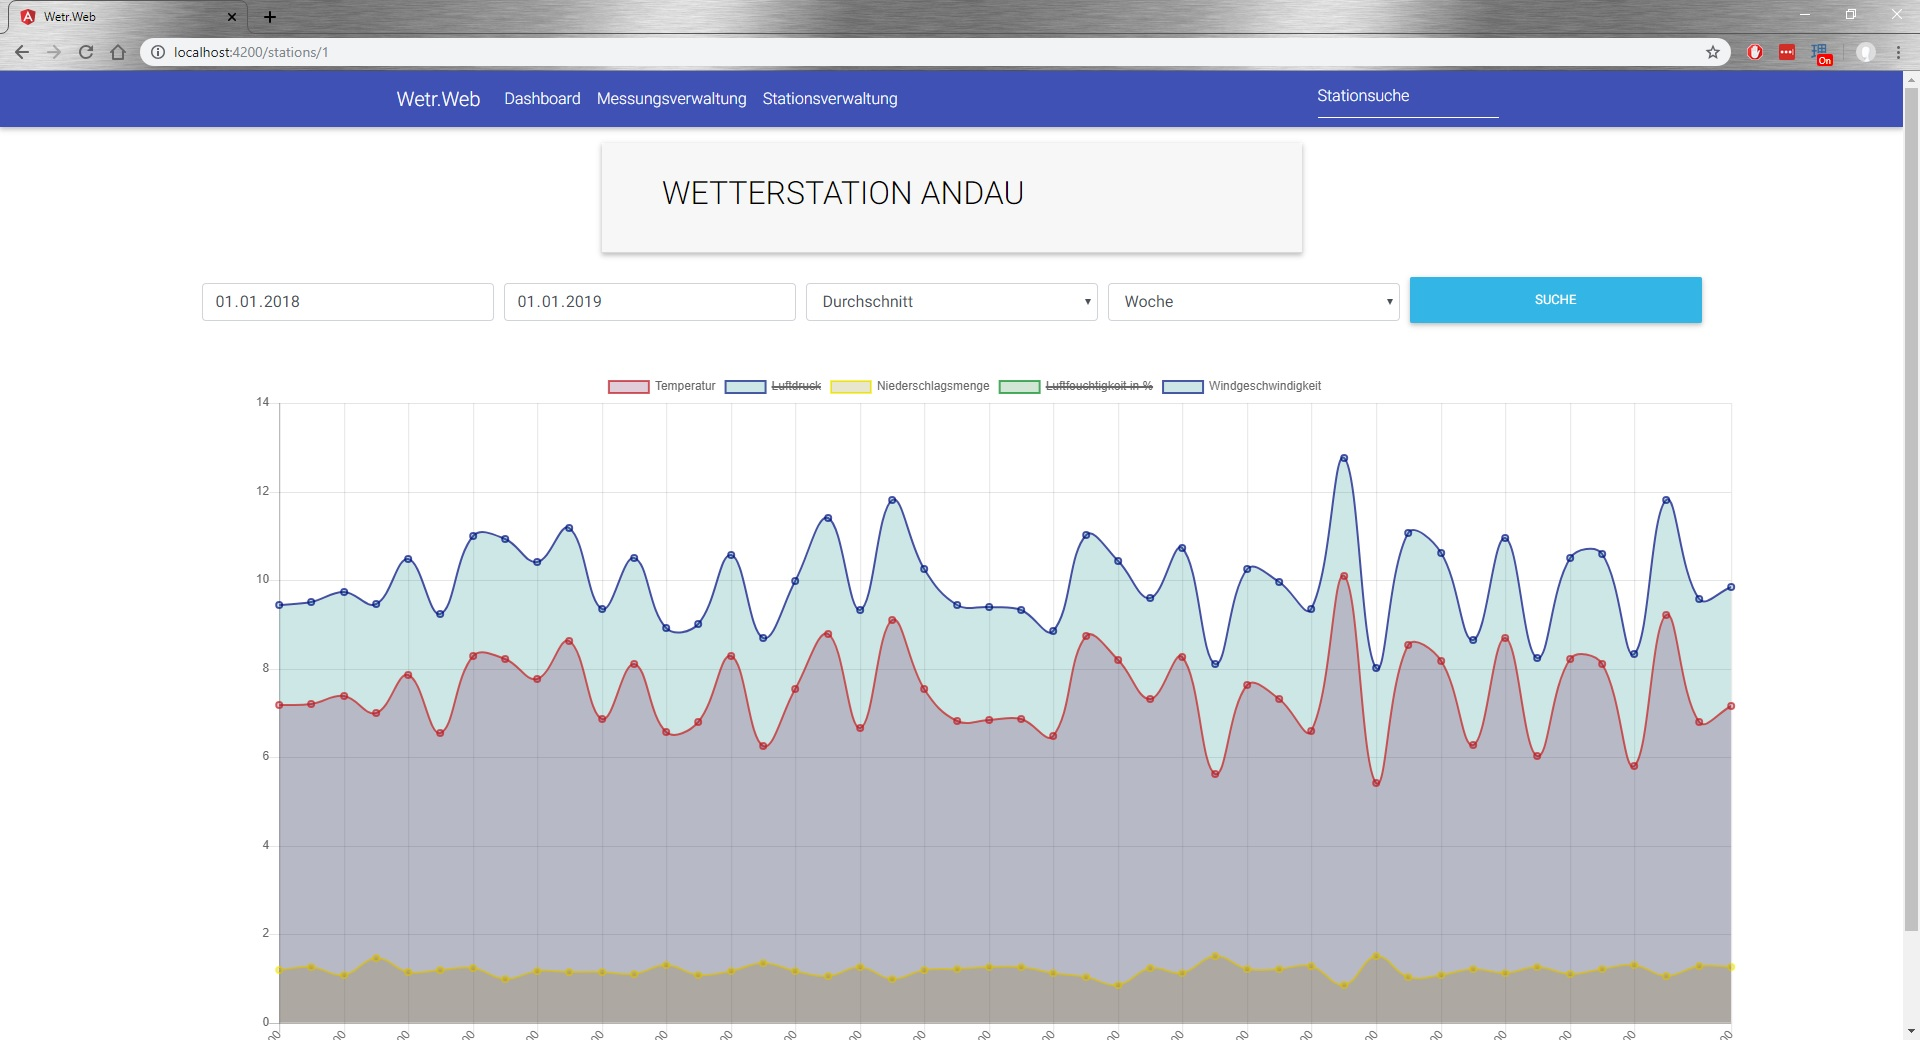
\includegraphics[width=\textwidth]{./img/station-detail.jpg}
	\centering
\end{figure}
Hier gibt es außerdem die Möglichkeit für eingeloggte Benutzer eine Station zum Dashboard hinzuzufügen
\begin{figure}[H]
	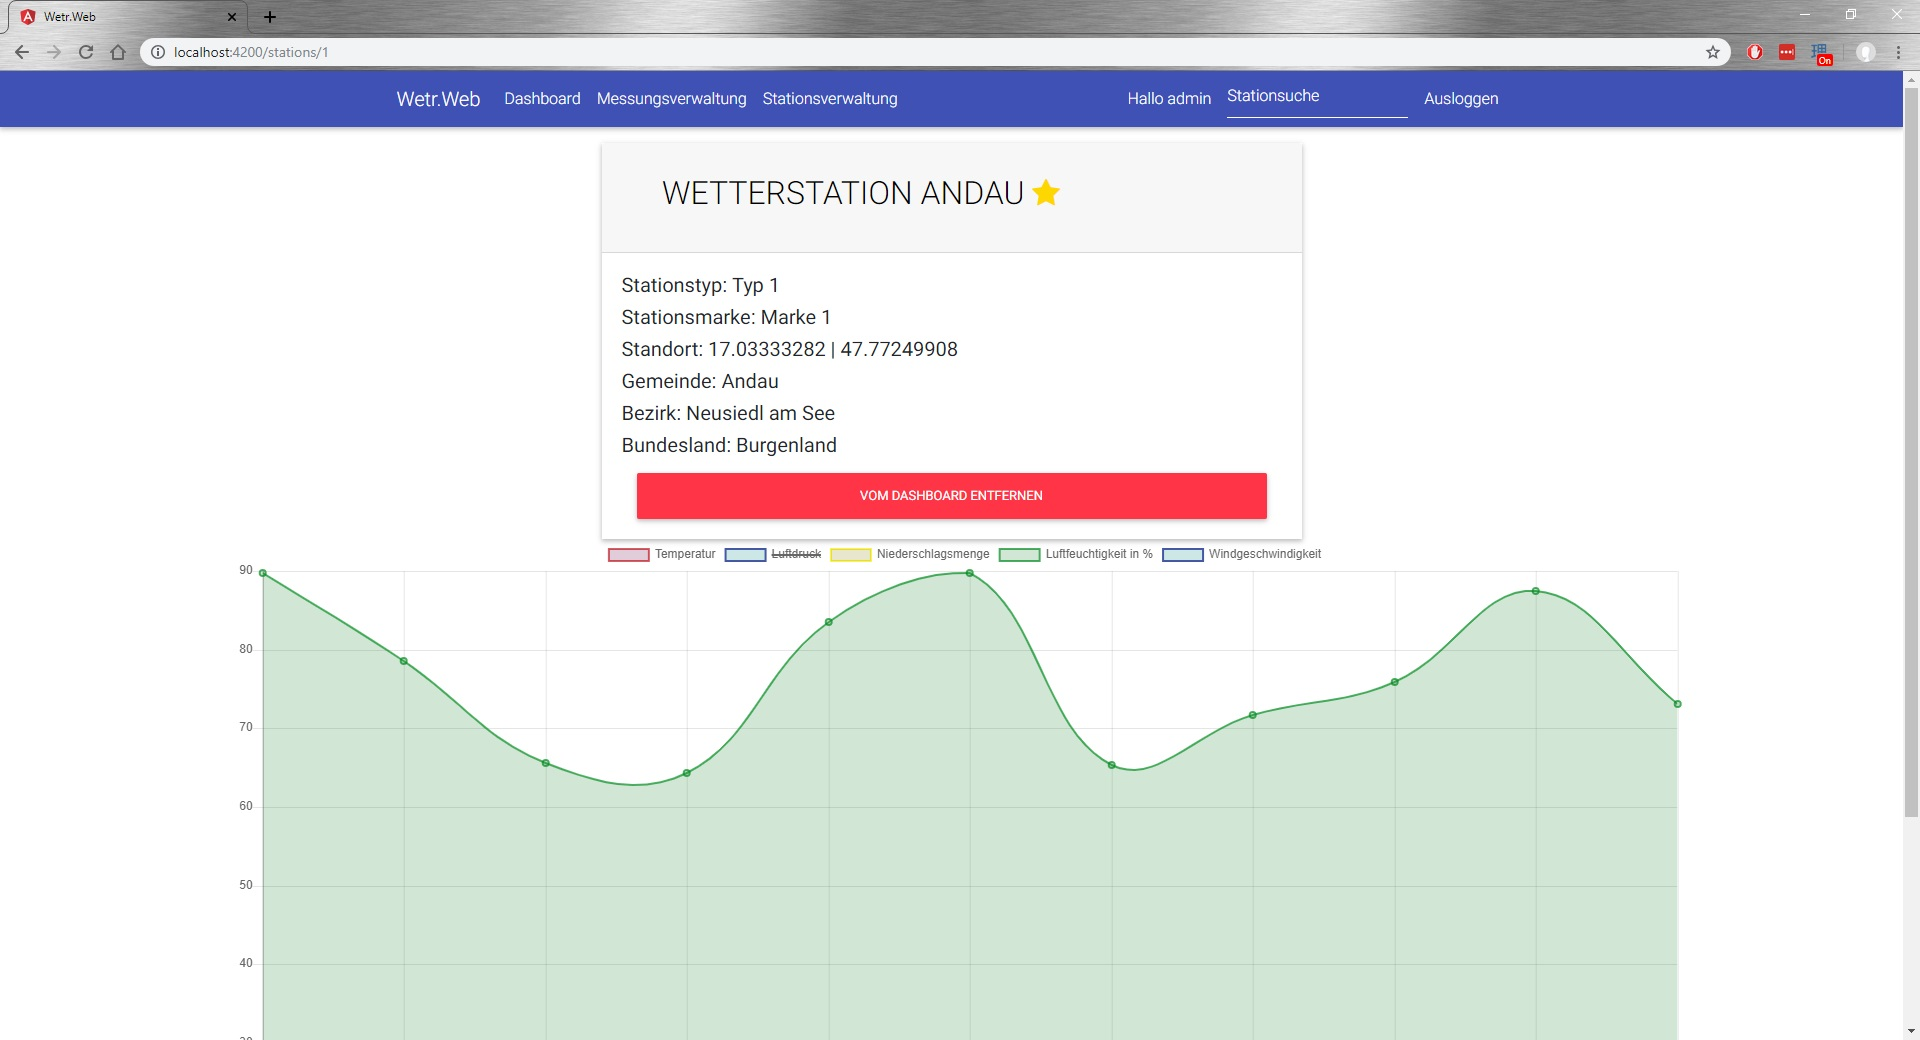
\includegraphics[width=\textwidth]{./img/station-detail1.jpg}
	\centering
\end{figure}
\subsection{Login}
Auf diese Komponente wird der Benutzer verwiesen wenn er Bereiche der Anwendung aufruft auf die nur eingeloggte Benutzer Zugriff haben.
\begin{figure}[H]
	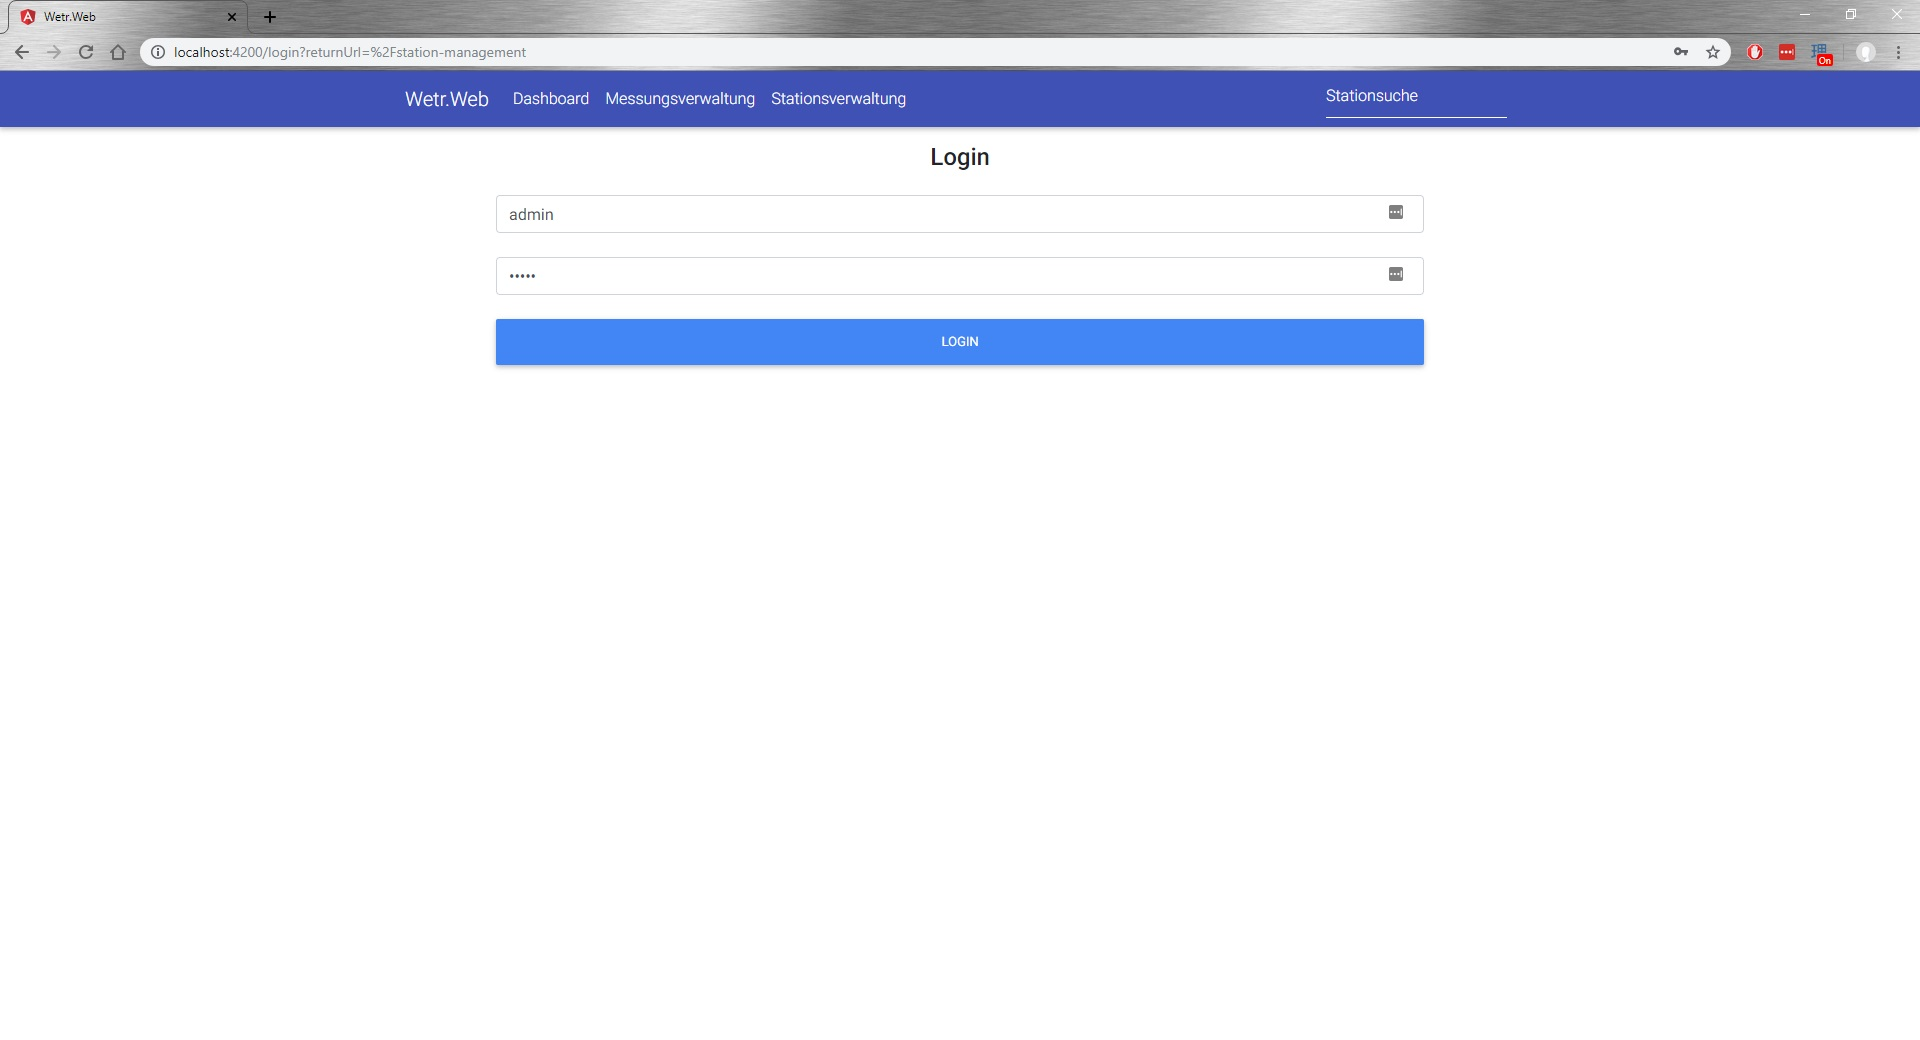
\includegraphics[width=\textwidth]{./img/login.jpg}
	\centering
\end{figure}
\end{document}
